% Created by tikzDevice version 0.12.3.1 on 2021-09-02 16:15:40
% !TEX encoding = UTF-8 Unicode
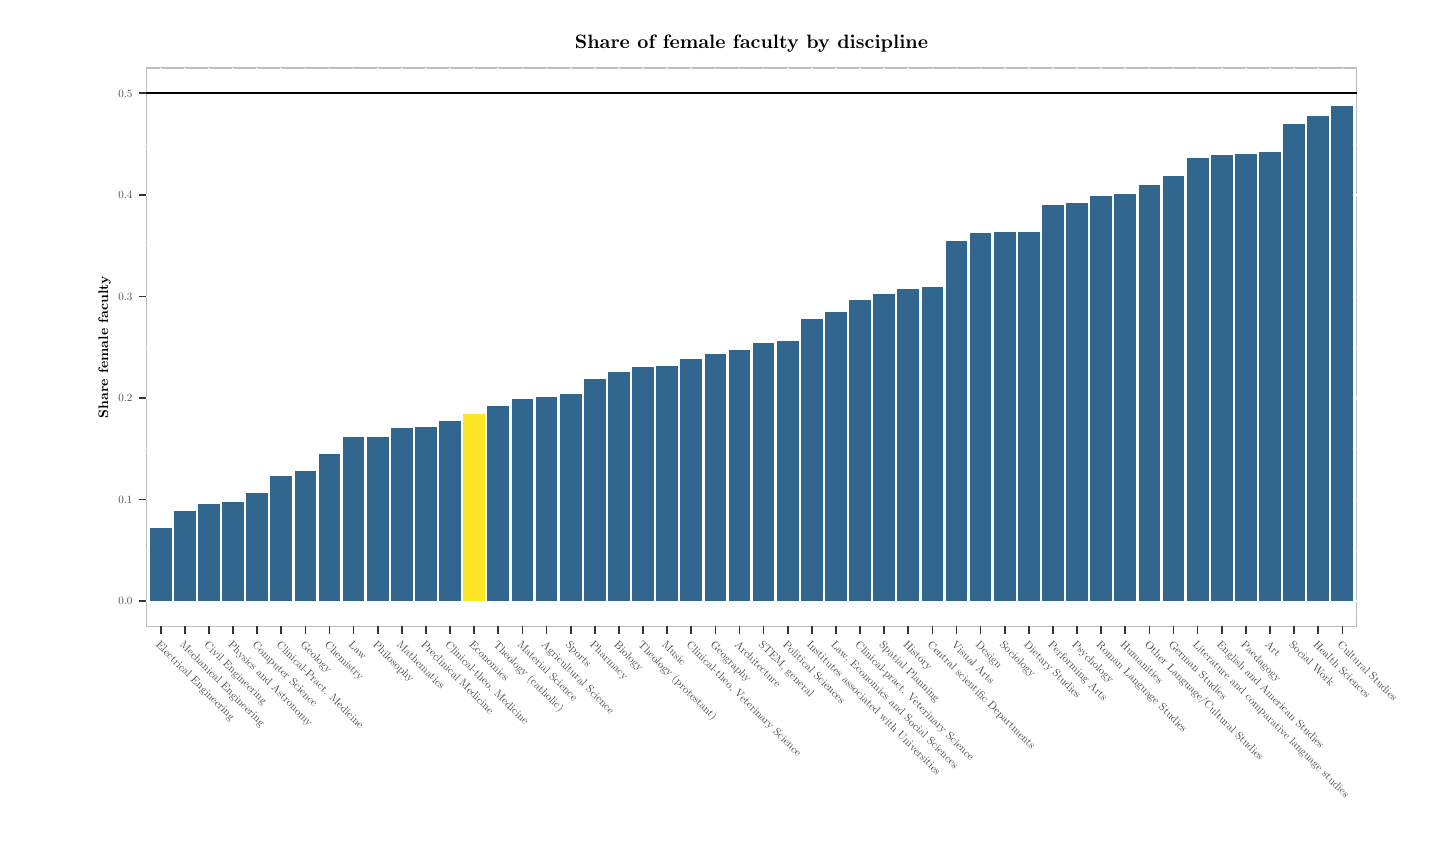
\begin{tikzpicture}[x=1pt,y=1pt]
\definecolor{fillColor}{RGB}{255,255,255}
\path[use as bounding box,fill=fillColor] (0,0) rectangle (505.89,289.08);
\begin{scope}
\path[clip] (  0.00,  0.00) rectangle (505.89,289.08);
\definecolor{drawColor}{RGB}{255,255,255}

\path[draw=drawColor,line width= 0.6pt,line join=round,line cap=round,fill=fillColor] (  0.00,  0.00) rectangle (505.89,289.08);
\end{scope}
\begin{scope}
\path[clip] ( 42.84, 72.70) rectangle (480.28,274.54);
\definecolor{drawColor}{RGB}{190,190,190}
\definecolor{fillColor}{RGB}{255,255,255}

\path[draw=drawColor,line width= 0.6pt,line join=round,line cap=round,fill=fillColor] ( 42.84, 72.70) rectangle (480.28,274.54);
\definecolor{drawColor}{RGB}{255,255,255}

\path[draw=drawColor,line width= 0.3pt,line join=round] ( 42.84,100.22) --
	(480.28,100.22);

\path[draw=drawColor,line width= 0.3pt,line join=round] ( 42.84,136.92) --
	(480.28,136.92);

\path[draw=drawColor,line width= 0.3pt,line join=round] ( 42.84,173.62) --
	(480.28,173.62);

\path[draw=drawColor,line width= 0.3pt,line join=round] ( 42.84,210.32) --
	(480.28,210.32);

\path[draw=drawColor,line width= 0.3pt,line join=round] ( 42.84,247.02) --
	(480.28,247.02);

\path[draw=drawColor,line width= 0.6pt,line join=round] ( 42.84, 81.87) --
	(480.28, 81.87);

\path[draw=drawColor,line width= 0.6pt,line join=round] ( 42.84,118.57) --
	(480.28,118.57);

\path[draw=drawColor,line width= 0.6pt,line join=round] ( 42.84,155.27) --
	(480.28,155.27);

\path[draw=drawColor,line width= 0.6pt,line join=round] ( 42.84,191.97) --
	(480.28,191.97);

\path[draw=drawColor,line width= 0.6pt,line join=round] ( 42.84,228.67) --
	(480.28,228.67);

\path[draw=drawColor,line width= 0.6pt,line join=round] ( 42.84,265.37) --
	(480.28,265.37);

\path[draw=drawColor,line width= 0.6pt,line join=round] ( 48.07, 72.70) --
	( 48.07,274.54);

\path[draw=drawColor,line width= 0.6pt,line join=round] ( 56.78, 72.70) --
	( 56.78,274.54);

\path[draw=drawColor,line width= 0.6pt,line join=round] ( 65.50, 72.70) --
	( 65.50,274.54);

\path[draw=drawColor,line width= 0.6pt,line join=round] ( 74.21, 72.70) --
	( 74.21,274.54);

\path[draw=drawColor,line width= 0.6pt,line join=round] ( 82.92, 72.70) --
	( 82.92,274.54);

\path[draw=drawColor,line width= 0.6pt,line join=round] ( 91.64, 72.70) --
	( 91.64,274.54);

\path[draw=drawColor,line width= 0.6pt,line join=round] (100.35, 72.70) --
	(100.35,274.54);

\path[draw=drawColor,line width= 0.6pt,line join=round] (109.07, 72.70) --
	(109.07,274.54);

\path[draw=drawColor,line width= 0.6pt,line join=round] (117.78, 72.70) --
	(117.78,274.54);

\path[draw=drawColor,line width= 0.6pt,line join=round] (126.49, 72.70) --
	(126.49,274.54);

\path[draw=drawColor,line width= 0.6pt,line join=round] (135.21, 72.70) --
	(135.21,274.54);

\path[draw=drawColor,line width= 0.6pt,line join=round] (143.92, 72.70) --
	(143.92,274.54);

\path[draw=drawColor,line width= 0.6pt,line join=round] (152.64, 72.70) --
	(152.64,274.54);

\path[draw=drawColor,line width= 0.6pt,line join=round] (161.35, 72.70) --
	(161.35,274.54);

\path[draw=drawColor,line width= 0.6pt,line join=round] (170.06, 72.70) --
	(170.06,274.54);

\path[draw=drawColor,line width= 0.6pt,line join=round] (178.78, 72.70) --
	(178.78,274.54);

\path[draw=drawColor,line width= 0.6pt,line join=round] (187.49, 72.70) --
	(187.49,274.54);

\path[draw=drawColor,line width= 0.6pt,line join=round] (196.21, 72.70) --
	(196.21,274.54);

\path[draw=drawColor,line width= 0.6pt,line join=round] (204.92, 72.70) --
	(204.92,274.54);

\path[draw=drawColor,line width= 0.6pt,line join=round] (213.63, 72.70) --
	(213.63,274.54);

\path[draw=drawColor,line width= 0.6pt,line join=round] (222.35, 72.70) --
	(222.35,274.54);

\path[draw=drawColor,line width= 0.6pt,line join=round] (231.06, 72.70) --
	(231.06,274.54);

\path[draw=drawColor,line width= 0.6pt,line join=round] (239.78, 72.70) --
	(239.78,274.54);

\path[draw=drawColor,line width= 0.6pt,line join=round] (248.49, 72.70) --
	(248.49,274.54);

\path[draw=drawColor,line width= 0.6pt,line join=round] (257.20, 72.70) --
	(257.20,274.54);

\path[draw=drawColor,line width= 0.6pt,line join=round] (265.92, 72.70) --
	(265.92,274.54);

\path[draw=drawColor,line width= 0.6pt,line join=round] (274.63, 72.70) --
	(274.63,274.54);

\path[draw=drawColor,line width= 0.6pt,line join=round] (283.35, 72.70) --
	(283.35,274.54);

\path[draw=drawColor,line width= 0.6pt,line join=round] (292.06, 72.70) --
	(292.06,274.54);

\path[draw=drawColor,line width= 0.6pt,line join=round] (300.77, 72.70) --
	(300.77,274.54);

\path[draw=drawColor,line width= 0.6pt,line join=round] (309.49, 72.70) --
	(309.49,274.54);

\path[draw=drawColor,line width= 0.6pt,line join=round] (318.20, 72.70) --
	(318.20,274.54);

\path[draw=drawColor,line width= 0.6pt,line join=round] (326.92, 72.70) --
	(326.92,274.54);

\path[draw=drawColor,line width= 0.6pt,line join=round] (335.63, 72.70) --
	(335.63,274.54);

\path[draw=drawColor,line width= 0.6pt,line join=round] (344.34, 72.70) --
	(344.34,274.54);

\path[draw=drawColor,line width= 0.6pt,line join=round] (353.06, 72.70) --
	(353.06,274.54);

\path[draw=drawColor,line width= 0.6pt,line join=round] (361.77, 72.70) --
	(361.77,274.54);

\path[draw=drawColor,line width= 0.6pt,line join=round] (370.49, 72.70) --
	(370.49,274.54);

\path[draw=drawColor,line width= 0.6pt,line join=round] (379.20, 72.70) --
	(379.20,274.54);

\path[draw=drawColor,line width= 0.6pt,line join=round] (387.91, 72.70) --
	(387.91,274.54);

\path[draw=drawColor,line width= 0.6pt,line join=round] (396.63, 72.70) --
	(396.63,274.54);

\path[draw=drawColor,line width= 0.6pt,line join=round] (405.34, 72.70) --
	(405.34,274.54);

\path[draw=drawColor,line width= 0.6pt,line join=round] (414.06, 72.70) --
	(414.06,274.54);

\path[draw=drawColor,line width= 0.6pt,line join=round] (422.77, 72.70) --
	(422.77,274.54);

\path[draw=drawColor,line width= 0.6pt,line join=round] (431.48, 72.70) --
	(431.48,274.54);

\path[draw=drawColor,line width= 0.6pt,line join=round] (440.20, 72.70) --
	(440.20,274.54);

\path[draw=drawColor,line width= 0.6pt,line join=round] (448.91, 72.70) --
	(448.91,274.54);

\path[draw=drawColor,line width= 0.6pt,line join=round] (457.63, 72.70) --
	(457.63,274.54);

\path[draw=drawColor,line width= 0.6pt,line join=round] (466.34, 72.70) --
	(466.34,274.54);

\path[draw=drawColor,line width= 0.6pt,line join=round] (475.05, 72.70) --
	(475.05,274.54);
\definecolor{fillColor}{RGB}{49,103,142}

\path[fill=fillColor] (392.71, 81.87) rectangle (400.55,228.91);

\path[fill=fillColor] (218.43, 81.87) rectangle (226.27,166.57);

\path[fill=fillColor] (166.14, 81.87) rectangle (173.99,152.49);

\path[fill=fillColor] (122.57, 81.87) rectangle (130.42,141.19);

\path[fill=fillColor] (314.28, 81.87) rectangle (322.12,194.47);

\path[fill=fillColor] (418.85, 81.87) rectangle (426.69,241.89);

\path[fill=fillColor] (410.13, 81.87) rectangle (417.98,235.47);

\path[fill=fillColor] (427.56, 81.87) rectangle (435.41,243.09);

\path[fill=fillColor] (383.99, 81.87) rectangle (391.84,228.12);

\path[fill=fillColor] (401.42, 81.87) rectangle (409.26,232.33);

\path[fill=fillColor] (471.13, 81.87) rectangle (478.98,260.73);

\path[fill=fillColor] (192.28, 81.87) rectangle (200.13,156.69);

\path[fill=fillColor] (288.14, 81.87) rectangle (295.98,186.25);

\path[fill=fillColor] (270.71, 81.87) rectangle (278.55,176.03);

\path[fill=fillColor] (349.14, 81.87) rectangle (356.98,215.30);

\path[fill=fillColor] (453.70, 81.87) rectangle (461.55,254.43);

\path[fill=fillColor] (113.86, 81.87) rectangle (121.70,141.10);
\definecolor{fillColor}{RGB}{253,231,37}

\path[fill=fillColor] (157.43, 81.87) rectangle (165.27,149.32);
\definecolor{fillColor}{RGB}{49,103,142}

\path[fill=fillColor] (375.28, 81.87) rectangle (383.12,225.69);

\path[fill=fillColor] (436.28, 81.87) rectangle (444.12,243.36);

\path[fill=fillColor] (262.00, 81.87) rectangle (269.84,175.08);

\path[fill=fillColor] (131.29, 81.87) rectangle (139.13,144.58);

\path[fill=fillColor] ( 70.29, 81.87) rectangle ( 78.13,117.69);

\path[fill=fillColor] (105.14, 81.87) rectangle (112.99,134.95);

\path[fill=fillColor] (201.00, 81.87) rectangle (208.84,162.12);

\path[fill=fillColor] (209.71, 81.87) rectangle (217.56,164.52);

\path[fill=fillColor] ( 96.43, 81.87) rectangle (104.27,128.98);

\path[fill=fillColor] (244.57, 81.87) rectangle (252.41,171.21);

\path[fill=fillColor] (462.42, 81.87) rectangle (470.26,257.02);

\path[fill=fillColor] (140.00, 81.87) rectangle (147.84,144.80);

\path[fill=fillColor] (148.71, 81.87) rectangle (156.56,147.01);

\path[fill=fillColor] ( 87.72, 81.87) rectangle ( 95.56,127.23);

\path[fill=fillColor] (235.85, 81.87) rectangle (243.70,169.23);

\path[fill=fillColor] (296.85, 81.87) rectangle (304.70,190.56);

\path[fill=fillColor] (183.57, 81.87) rectangle (191.41,155.76);

\path[fill=fillColor] (357.85, 81.87) rectangle (365.69,215.40);

\path[fill=fillColor] ( 52.86, 81.87) rectangle ( 60.70,114.44);

\path[fill=fillColor] ( 44.15, 81.87) rectangle ( 51.99,108.46);

\path[fill=fillColor] (253.28, 81.87) rectangle (261.13,172.75);

\path[fill=fillColor] (305.57, 81.87) rectangle (313.41,192.77);

\path[fill=fillColor] ( 61.57, 81.87) rectangle ( 69.42,117.13);

\path[fill=fillColor] ( 79.00, 81.87) rectangle ( 86.85,120.87);

\path[fill=fillColor] (174.86, 81.87) rectangle (182.70,154.93);

\path[fill=fillColor] (444.99, 81.87) rectangle (452.83,244.15);

\path[fill=fillColor] (331.71, 81.87) rectangle (339.55,212.05);

\path[fill=fillColor] (340.42, 81.87) rectangle (348.27,214.86);

\path[fill=fillColor] (366.56, 81.87) rectangle (374.41,225.16);

\path[fill=fillColor] (227.14, 81.87) rectangle (234.98,166.83);

\path[fill=fillColor] (322.99, 81.87) rectangle (330.84,195.33);

\path[fill=fillColor] (279.42, 81.87) rectangle (287.27,183.95);
\definecolor{drawColor}{RGB}{0,0,0}

\path[draw=drawColor,line width= 0.6pt,line join=round] ( 42.84,265.37) -- (480.28,265.37);
\end{scope}
\begin{scope}
\path[clip] (  0.00,  0.00) rectangle (505.89,289.08);
\definecolor{drawColor}{gray}{0.30}

\node[text=drawColor,anchor=base east,inner sep=0pt, outer sep=0pt, scale=  0.40] at ( 37.89, 80.50) {0.0};

\node[text=drawColor,anchor=base east,inner sep=0pt, outer sep=0pt, scale=  0.40] at ( 37.89,117.20) {0.1};

\node[text=drawColor,anchor=base east,inner sep=0pt, outer sep=0pt, scale=  0.40] at ( 37.89,153.89) {0.2};

\node[text=drawColor,anchor=base east,inner sep=0pt, outer sep=0pt, scale=  0.40] at ( 37.89,190.59) {0.3};

\node[text=drawColor,anchor=base east,inner sep=0pt, outer sep=0pt, scale=  0.40] at ( 37.89,227.29) {0.4};

\node[text=drawColor,anchor=base east,inner sep=0pt, outer sep=0pt, scale=  0.40] at ( 37.89,263.99) {0.5};
\end{scope}
\begin{scope}
\path[clip] (  0.00,  0.00) rectangle (505.89,289.08);
\definecolor{drawColor}{gray}{0.20}

\path[draw=drawColor,line width= 0.6pt,line join=round] ( 40.09, 81.87) --
	( 42.84, 81.87);

\path[draw=drawColor,line width= 0.6pt,line join=round] ( 40.09,118.57) --
	( 42.84,118.57);

\path[draw=drawColor,line width= 0.6pt,line join=round] ( 40.09,155.27) --
	( 42.84,155.27);

\path[draw=drawColor,line width= 0.6pt,line join=round] ( 40.09,191.97) --
	( 42.84,191.97);

\path[draw=drawColor,line width= 0.6pt,line join=round] ( 40.09,228.67) --
	( 42.84,228.67);

\path[draw=drawColor,line width= 0.6pt,line join=round] ( 40.09,265.37) --
	( 42.84,265.37);
\end{scope}
\begin{scope}
\path[clip] (  0.00,  0.00) rectangle (505.89,289.08);
\definecolor{drawColor}{gray}{0.20}

\path[draw=drawColor,line width= 0.6pt,line join=round] ( 48.07, 69.95) --
	( 48.07, 72.70);

\path[draw=drawColor,line width= 0.6pt,line join=round] ( 56.78, 69.95) --
	( 56.78, 72.70);

\path[draw=drawColor,line width= 0.6pt,line join=round] ( 65.50, 69.95) --
	( 65.50, 72.70);

\path[draw=drawColor,line width= 0.6pt,line join=round] ( 74.21, 69.95) --
	( 74.21, 72.70);

\path[draw=drawColor,line width= 0.6pt,line join=round] ( 82.92, 69.95) --
	( 82.92, 72.70);

\path[draw=drawColor,line width= 0.6pt,line join=round] ( 91.64, 69.95) --
	( 91.64, 72.70);

\path[draw=drawColor,line width= 0.6pt,line join=round] (100.35, 69.95) --
	(100.35, 72.70);

\path[draw=drawColor,line width= 0.6pt,line join=round] (109.07, 69.95) --
	(109.07, 72.70);

\path[draw=drawColor,line width= 0.6pt,line join=round] (117.78, 69.95) --
	(117.78, 72.70);

\path[draw=drawColor,line width= 0.6pt,line join=round] (126.49, 69.95) --
	(126.49, 72.70);

\path[draw=drawColor,line width= 0.6pt,line join=round] (135.21, 69.95) --
	(135.21, 72.70);

\path[draw=drawColor,line width= 0.6pt,line join=round] (143.92, 69.95) --
	(143.92, 72.70);

\path[draw=drawColor,line width= 0.6pt,line join=round] (152.64, 69.95) --
	(152.64, 72.70);

\path[draw=drawColor,line width= 0.6pt,line join=round] (161.35, 69.95) --
	(161.35, 72.70);

\path[draw=drawColor,line width= 0.6pt,line join=round] (170.06, 69.95) --
	(170.06, 72.70);

\path[draw=drawColor,line width= 0.6pt,line join=round] (178.78, 69.95) --
	(178.78, 72.70);

\path[draw=drawColor,line width= 0.6pt,line join=round] (187.49, 69.95) --
	(187.49, 72.70);

\path[draw=drawColor,line width= 0.6pt,line join=round] (196.21, 69.95) --
	(196.21, 72.70);

\path[draw=drawColor,line width= 0.6pt,line join=round] (204.92, 69.95) --
	(204.92, 72.70);

\path[draw=drawColor,line width= 0.6pt,line join=round] (213.63, 69.95) --
	(213.63, 72.70);

\path[draw=drawColor,line width= 0.6pt,line join=round] (222.35, 69.95) --
	(222.35, 72.70);

\path[draw=drawColor,line width= 0.6pt,line join=round] (231.06, 69.95) --
	(231.06, 72.70);

\path[draw=drawColor,line width= 0.6pt,line join=round] (239.78, 69.95) --
	(239.78, 72.70);

\path[draw=drawColor,line width= 0.6pt,line join=round] (248.49, 69.95) --
	(248.49, 72.70);

\path[draw=drawColor,line width= 0.6pt,line join=round] (257.20, 69.95) --
	(257.20, 72.70);

\path[draw=drawColor,line width= 0.6pt,line join=round] (265.92, 69.95) --
	(265.92, 72.70);

\path[draw=drawColor,line width= 0.6pt,line join=round] (274.63, 69.95) --
	(274.63, 72.70);

\path[draw=drawColor,line width= 0.6pt,line join=round] (283.35, 69.95) --
	(283.35, 72.70);

\path[draw=drawColor,line width= 0.6pt,line join=round] (292.06, 69.95) --
	(292.06, 72.70);

\path[draw=drawColor,line width= 0.6pt,line join=round] (300.77, 69.95) --
	(300.77, 72.70);

\path[draw=drawColor,line width= 0.6pt,line join=round] (309.49, 69.95) --
	(309.49, 72.70);

\path[draw=drawColor,line width= 0.6pt,line join=round] (318.20, 69.95) --
	(318.20, 72.70);

\path[draw=drawColor,line width= 0.6pt,line join=round] (326.92, 69.95) --
	(326.92, 72.70);

\path[draw=drawColor,line width= 0.6pt,line join=round] (335.63, 69.95) --
	(335.63, 72.70);

\path[draw=drawColor,line width= 0.6pt,line join=round] (344.34, 69.95) --
	(344.34, 72.70);

\path[draw=drawColor,line width= 0.6pt,line join=round] (353.06, 69.95) --
	(353.06, 72.70);

\path[draw=drawColor,line width= 0.6pt,line join=round] (361.77, 69.95) --
	(361.77, 72.70);

\path[draw=drawColor,line width= 0.6pt,line join=round] (370.49, 69.95) --
	(370.49, 72.70);

\path[draw=drawColor,line width= 0.6pt,line join=round] (379.20, 69.95) --
	(379.20, 72.70);

\path[draw=drawColor,line width= 0.6pt,line join=round] (387.91, 69.95) --
	(387.91, 72.70);

\path[draw=drawColor,line width= 0.6pt,line join=round] (396.63, 69.95) --
	(396.63, 72.70);

\path[draw=drawColor,line width= 0.6pt,line join=round] (405.34, 69.95) --
	(405.34, 72.70);

\path[draw=drawColor,line width= 0.6pt,line join=round] (414.06, 69.95) --
	(414.06, 72.70);

\path[draw=drawColor,line width= 0.6pt,line join=round] (422.77, 69.95) --
	(422.77, 72.70);

\path[draw=drawColor,line width= 0.6pt,line join=round] (431.48, 69.95) --
	(431.48, 72.70);

\path[draw=drawColor,line width= 0.6pt,line join=round] (440.20, 69.95) --
	(440.20, 72.70);

\path[draw=drawColor,line width= 0.6pt,line join=round] (448.91, 69.95) --
	(448.91, 72.70);

\path[draw=drawColor,line width= 0.6pt,line join=round] (457.63, 69.95) --
	(457.63, 72.70);

\path[draw=drawColor,line width= 0.6pt,line join=round] (466.34, 69.95) --
	(466.34, 72.70);

\path[draw=drawColor,line width= 0.6pt,line join=round] (475.05, 69.95) --
	(475.05, 72.70);
\end{scope}
\begin{scope}
\path[clip] (  0.00,  0.00) rectangle (505.89,289.08);
\definecolor{drawColor}{gray}{0.30}

\node[text=drawColor,rotate=-45.00,anchor=base west,inner sep=0pt, outer sep=0pt, scale=  0.40] at ( 46.12, 65.80) {Electrical Engineering};

\node[text=drawColor,rotate=-45.00,anchor=base west,inner sep=0pt, outer sep=0pt, scale=  0.40] at ( 54.83, 65.80) {Mechanical Engineering};

\node[text=drawColor,rotate=-45.00,anchor=base west,inner sep=0pt, outer sep=0pt, scale=  0.40] at ( 63.55, 65.80) {Civil Engineering};

\node[text=drawColor,rotate=-45.00,anchor=base west,inner sep=0pt, outer sep=0pt, scale=  0.40] at ( 72.26, 65.80) {Physics and Astronomy};

\node[text=drawColor,rotate=-45.00,anchor=base west,inner sep=0pt, outer sep=0pt, scale=  0.40] at ( 80.98, 65.80) {Computer Science};

\node[text=drawColor,rotate=-45.00,anchor=base west,inner sep=0pt, outer sep=0pt, scale=  0.40] at ( 89.69, 65.80) {Clinical-Pract. Medicine};

\node[text=drawColor,rotate=-45.00,anchor=base west,inner sep=0pt, outer sep=0pt, scale=  0.40] at ( 98.40, 65.80) {Geology};

\node[text=drawColor,rotate=-45.00,anchor=base west,inner sep=0pt, outer sep=0pt, scale=  0.40] at (107.12, 65.80) {Chemistry};

\node[text=drawColor,rotate=-45.00,anchor=base west,inner sep=0pt, outer sep=0pt, scale=  0.40] at (115.83, 65.80) {Law};

\node[text=drawColor,rotate=-45.00,anchor=base west,inner sep=0pt, outer sep=0pt, scale=  0.40] at (124.55, 65.80) {Philosophy};

\node[text=drawColor,rotate=-45.00,anchor=base west,inner sep=0pt, outer sep=0pt, scale=  0.40] at (133.26, 65.80) {Mathematics};

\node[text=drawColor,rotate=-45.00,anchor=base west,inner sep=0pt, outer sep=0pt, scale=  0.40] at (141.97, 65.80) {Preclinical Medicine};

\node[text=drawColor,rotate=-45.00,anchor=base west,inner sep=0pt, outer sep=0pt, scale=  0.40] at (150.69, 65.80) {Clinical-theo. Medicine};

\node[text=drawColor,rotate=-45.00,anchor=base west,inner sep=0pt, outer sep=0pt, scale=  0.40] at (159.40, 65.80) {Economics};

\node[text=drawColor,rotate=-45.00,anchor=base west,inner sep=0pt, outer sep=0pt, scale=  0.40] at (168.12, 65.80) {Theology (catholic)};

\node[text=drawColor,rotate=-45.00,anchor=base west,inner sep=0pt, outer sep=0pt, scale=  0.40] at (176.83, 65.80) {Material Science};

\node[text=drawColor,rotate=-45.00,anchor=base west,inner sep=0pt, outer sep=0pt, scale=  0.40] at (185.54, 65.80) {Agricultural Science};

\node[text=drawColor,rotate=-45.00,anchor=base west,inner sep=0pt, outer sep=0pt, scale=  0.40] at (194.26, 65.80) {Sports};

\node[text=drawColor,rotate=-45.00,anchor=base west,inner sep=0pt, outer sep=0pt, scale=  0.40] at (202.97, 65.80) {Pharmacy};

\node[text=drawColor,rotate=-45.00,anchor=base west,inner sep=0pt, outer sep=0pt, scale=  0.40] at (211.69, 65.80) {Biology};

\node[text=drawColor,rotate=-45.00,anchor=base west,inner sep=0pt, outer sep=0pt, scale=  0.40] at (220.40, 65.80) {Theology (protestant)};

\node[text=drawColor,rotate=-45.00,anchor=base west,inner sep=0pt, outer sep=0pt, scale=  0.40] at (229.11, 65.80) {Music};

\node[text=drawColor,rotate=-45.00,anchor=base west,inner sep=0pt, outer sep=0pt, scale=  0.40] at (237.83, 65.80) {Clinical-theo, Veterinary Science};

\node[text=drawColor,rotate=-45.00,anchor=base west,inner sep=0pt, outer sep=0pt, scale=  0.40] at (246.54, 65.80) {Geography};

\node[text=drawColor,rotate=-45.00,anchor=base west,inner sep=0pt, outer sep=0pt, scale=  0.40] at (255.26, 65.80) {Architecture};

\node[text=drawColor,rotate=-45.00,anchor=base west,inner sep=0pt, outer sep=0pt, scale=  0.40] at (263.97, 65.80) {STEM, general};

\node[text=drawColor,rotate=-45.00,anchor=base west,inner sep=0pt, outer sep=0pt, scale=  0.40] at (272.68, 65.80) {Political Sciences};

\node[text=drawColor,rotate=-45.00,anchor=base west,inner sep=0pt, outer sep=0pt, scale=  0.40] at (281.40, 65.80) {Institutes associated with Universities};

\node[text=drawColor,rotate=-45.00,anchor=base west,inner sep=0pt, outer sep=0pt, scale=  0.40] at (290.11, 65.80) {Law, Economics and Social Sciences};

\node[text=drawColor,rotate=-45.00,anchor=base west,inner sep=0pt, outer sep=0pt, scale=  0.40] at (298.83, 65.80) {Clinical-pract. Veterinary Science};

\node[text=drawColor,rotate=-45.00,anchor=base west,inner sep=0pt, outer sep=0pt, scale=  0.40] at (307.54, 65.80) {Spatial Planning};

\node[text=drawColor,rotate=-45.00,anchor=base west,inner sep=0pt, outer sep=0pt, scale=  0.40] at (316.25, 65.80) {History};

\node[text=drawColor,rotate=-45.00,anchor=base west,inner sep=0pt, outer sep=0pt, scale=  0.40] at (324.97, 65.80) {Central scientific Departments};

\node[text=drawColor,rotate=-45.00,anchor=base west,inner sep=0pt, outer sep=0pt, scale=  0.40] at (333.68, 65.80) {Visual Arts};

\node[text=drawColor,rotate=-45.00,anchor=base west,inner sep=0pt, outer sep=0pt, scale=  0.40] at (342.40, 65.80) {Design};

\node[text=drawColor,rotate=-45.00,anchor=base west,inner sep=0pt, outer sep=0pt, scale=  0.40] at (351.11, 65.80) {Sociology};

\node[text=drawColor,rotate=-45.00,anchor=base west,inner sep=0pt, outer sep=0pt, scale=  0.40] at (359.82, 65.80) {Dietary Studies};

\node[text=drawColor,rotate=-45.00,anchor=base west,inner sep=0pt, outer sep=0pt, scale=  0.40] at (368.54, 65.80) {Performing Arts};

\node[text=drawColor,rotate=-45.00,anchor=base west,inner sep=0pt, outer sep=0pt, scale=  0.40] at (377.25, 65.80) {Psychology};

\node[text=drawColor,rotate=-45.00,anchor=base west,inner sep=0pt, outer sep=0pt, scale=  0.40] at (385.97, 65.80) {Roman Language Studies};

\node[text=drawColor,rotate=-45.00,anchor=base west,inner sep=0pt, outer sep=0pt, scale=  0.40] at (394.68, 65.80) {Humanities};

\node[text=drawColor,rotate=-45.00,anchor=base west,inner sep=0pt, outer sep=0pt, scale=  0.40] at (403.39, 65.80) {Other Language/Cultural Studies};

\node[text=drawColor,rotate=-45.00,anchor=base west,inner sep=0pt, outer sep=0pt, scale=  0.40] at (412.11, 65.80) {German Studies};

\node[text=drawColor,rotate=-45.00,anchor=base west,inner sep=0pt, outer sep=0pt, scale=  0.40] at (420.82, 65.80) {Literature and comparative language studies};

\node[text=drawColor,rotate=-45.00,anchor=base west,inner sep=0pt, outer sep=0pt, scale=  0.40] at (429.54, 65.80) {English and American Studies};

\node[text=drawColor,rotate=-45.00,anchor=base west,inner sep=0pt, outer sep=0pt, scale=  0.40] at (438.25, 65.80) {Paedagogy};

\node[text=drawColor,rotate=-45.00,anchor=base west,inner sep=0pt, outer sep=0pt, scale=  0.40] at (446.96, 65.80) {Art};

\node[text=drawColor,rotate=-45.00,anchor=base west,inner sep=0pt, outer sep=0pt, scale=  0.40] at (455.68, 65.80) {Social Work};

\node[text=drawColor,rotate=-45.00,anchor=base west,inner sep=0pt, outer sep=0pt, scale=  0.40] at (464.39, 65.80) {Health Sciences};

\node[text=drawColor,rotate=-45.00,anchor=base west,inner sep=0pt, outer sep=0pt, scale=  0.40] at (473.11, 65.80) {Cultural Studies};
\end{scope}
\begin{scope}
\path[clip] (  0.00,  0.00) rectangle (505.89,289.08);
\definecolor{drawColor}{RGB}{0,0,0}

\node[text=drawColor,rotate= 90.00,anchor=base,inner sep=0pt, outer sep=0pt, scale=  0.50] at ( 29.06,173.62) {\bfseries Share female faculty};
\end{scope}
\begin{scope}
\path[clip] (  0.00,  0.00) rectangle (505.89,289.08);
\definecolor{drawColor}{RGB}{0,0,0}

\node[text=drawColor,anchor=base,inner sep=0pt, outer sep=0pt, scale=  0.70] at (261.56,281.40) {\bfseries Share of female faculty by discipline};
\end{scope}
\end{tikzpicture}
